% filename: ProgramPlotsSF.tex
\documentclass[11pt]{article}
\include{PhysNote}
\usepackage{srcltx}

\usepackage{ifpdf} % to switch between .epsf and .png file types for images (for compiling)
\usepackage{grffile} % so file.name.pdf (filename with a period in it) will be recognized as a PDF file

\title{Program Plots SF (``Supporting'' Folder)}
\author{Andrew Forrester}


\begin{document}
\maketitle
\tableofcontents


%\newpage
\section{Files}

\begin{comment}
plot_vlt_ThermStates_Dexp100_beta_Cc1.03_K0cTest.ps
splot_BrooksDonnelly_AlphaVsTP.ps
splot_BrooksDonnelly_RhoVsTP.ps
splot_fit_BrooksDonnelly_AlphaVsTP_4order.ps
splot_fit_BrooksDonnelly_AlphaVsTP_5order.ps
splot_fit_BrooksDonnelly_AlphaVsTP_6order.ps
splot_fit_BrooksDonnelly_RhoVsTP_4order.ps

plot_DelokFit0.png
plot_DelokFit1.png
plot_DelokFit2.png
plot_DelokFits.png
plot_DelokFit_test.png
\end{comment}

\squishlist
  \item \verb|plot_vlt_ThermStates_Dexp100_beta_Cc1.03_K0cTest.ps|
  \item \verb|splot_BrooksDonnelly_AlphaVsTP.ps|
  \item \verb|splot_fit_BrooksDonnelly_AlphaVsTP_4order.ps|
  \item \verb|splot_fit_BrooksDonnelly_AlphaVsTP_5order.ps|
  \item \verb|splot_fit_BrooksDonnelly_AlphaVsTP_6order.ps|
  \item \verb|splot_fit_BrooksDonnelly_RhoVsTP_4order.ps|
  \item \verb|plot_DelokFit0.png|
  \item \verb|plot_DelokFit1.png|
  \item \verb|plot_DelokFit2.png|
  \item \verb|plot_DelokFits.png|
\squishend



\section{Checking for Criticality of K0c}

\begin{center}
\begin{tabular}[\textwidth]{p{8.5cm}p{8.5cm}}
\ifpdf
  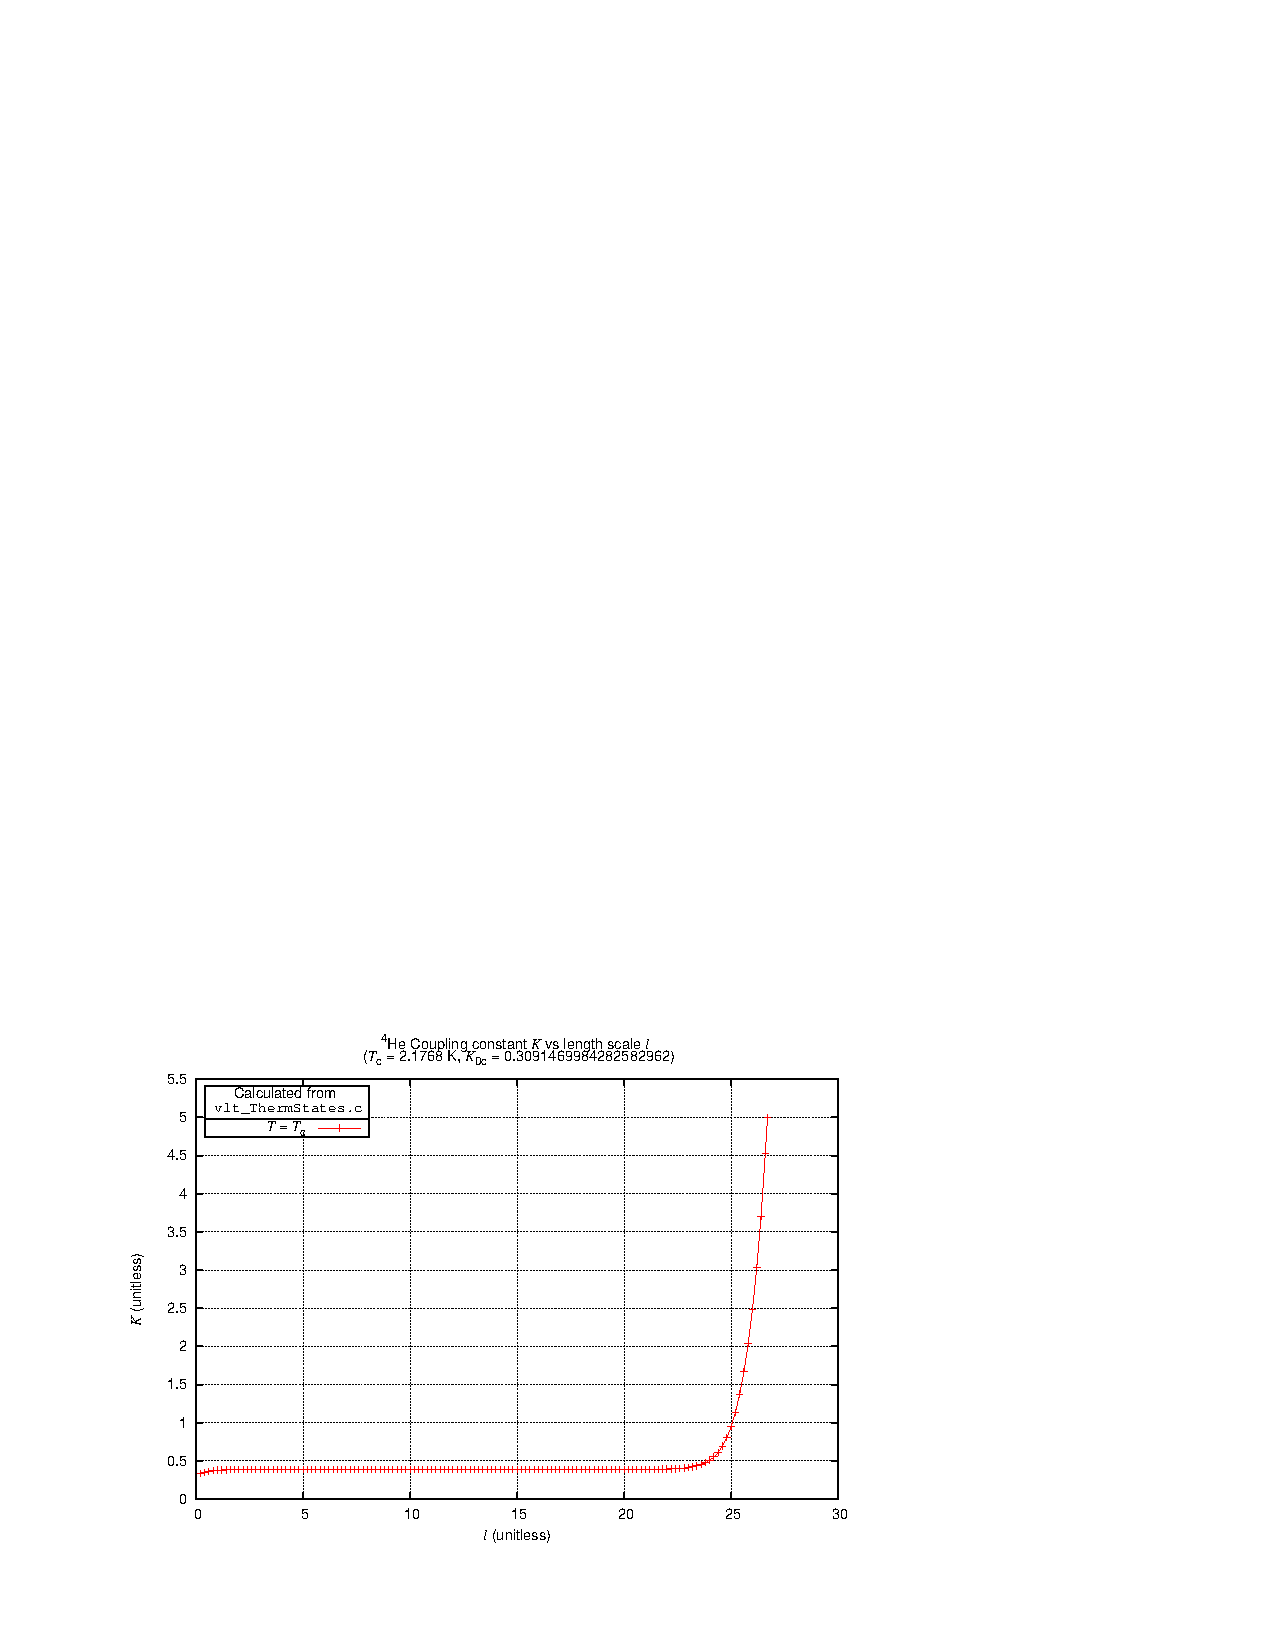
\includegraphics[width=8.5cm,viewport=54 53 410 300]{plot_vlt_ThermStates_Dexp100_beta_Cc1.03_K0cTest.pdf}\newline
  \verb|plot_vlt_ThermStates_Dexp100_beta_Cc1.03_K0cTest.pdf|
\else
  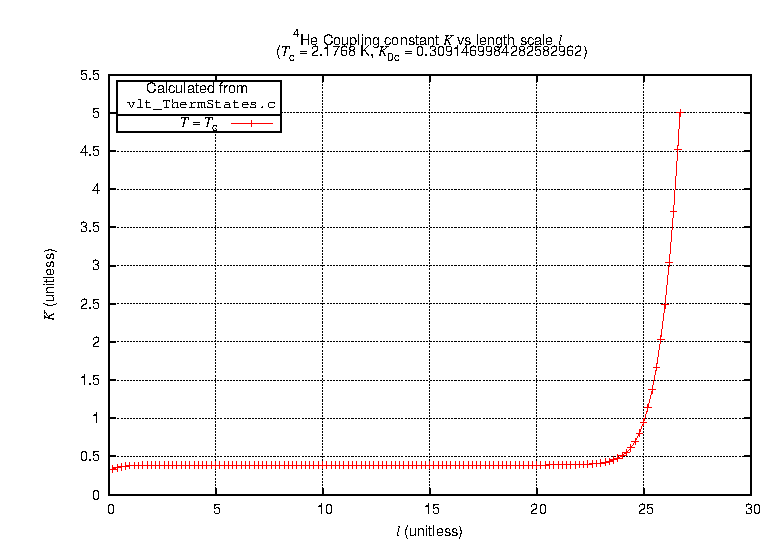
\includegraphics[width=8.5cm]{plot_vlt_ThermStates_Dexp100_beta_Cc1.03_K0cTest.ps}\newline
  \verb|plot_vlt_ThermStates_Dexp100_beta_Cc1.03_K0cTest.ps|
\fi
&
 \\
\end{tabular}
\end{center}



\section{Fits of Data from Literature}

\begin{center}
\begin{tabular}[\textwidth]{p{8.5cm}p{8.5cm}}
\ifpdf
  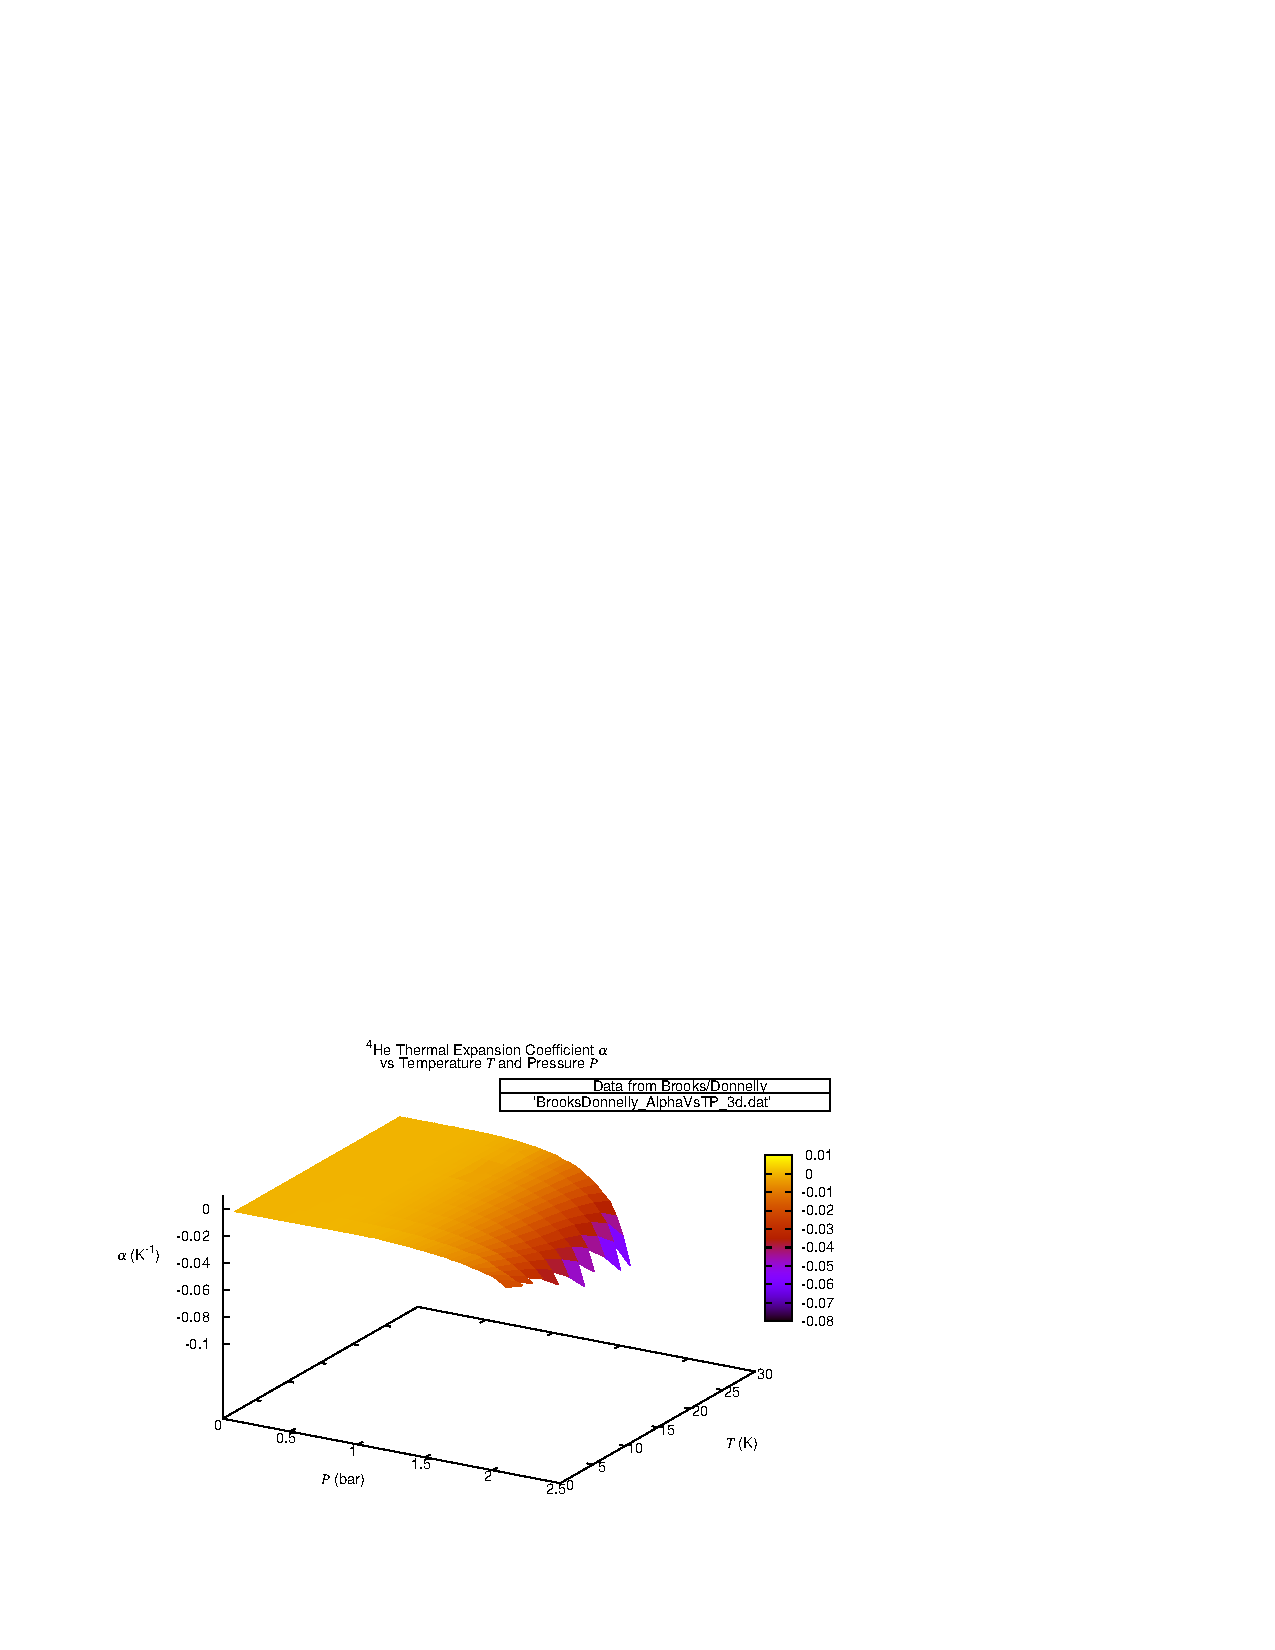
\includegraphics[width=8.5cm,viewport=54 53 410 300]{splot_BrooksDonnelly_AlphaVsTP.pdf}\newline
  \verb|splot_BrooksDonnelly_AlphaVsTP.pdf|
\else
  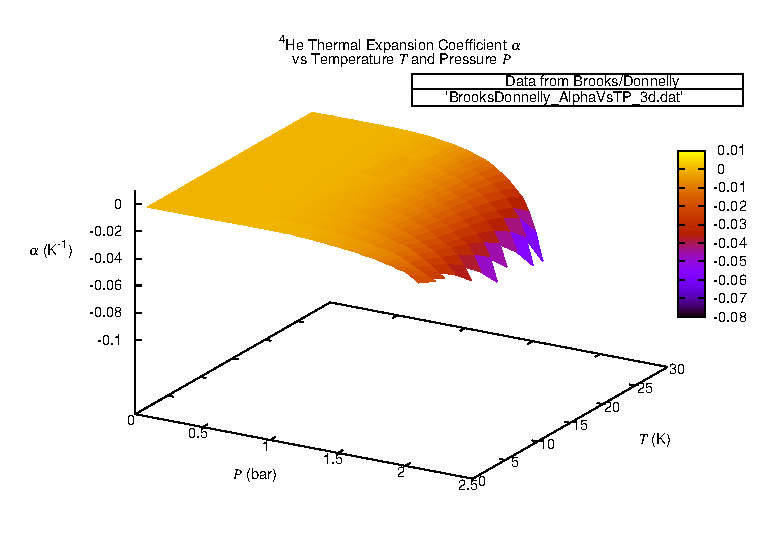
\includegraphics[width=8.5cm]{splot_BrooksDonnelly_AlphaVsTP.ps}\newline
  \verb|splot_BrooksDonnelly_AlphaVsTP.ps|
\fi
&
 \\
\ifpdf
  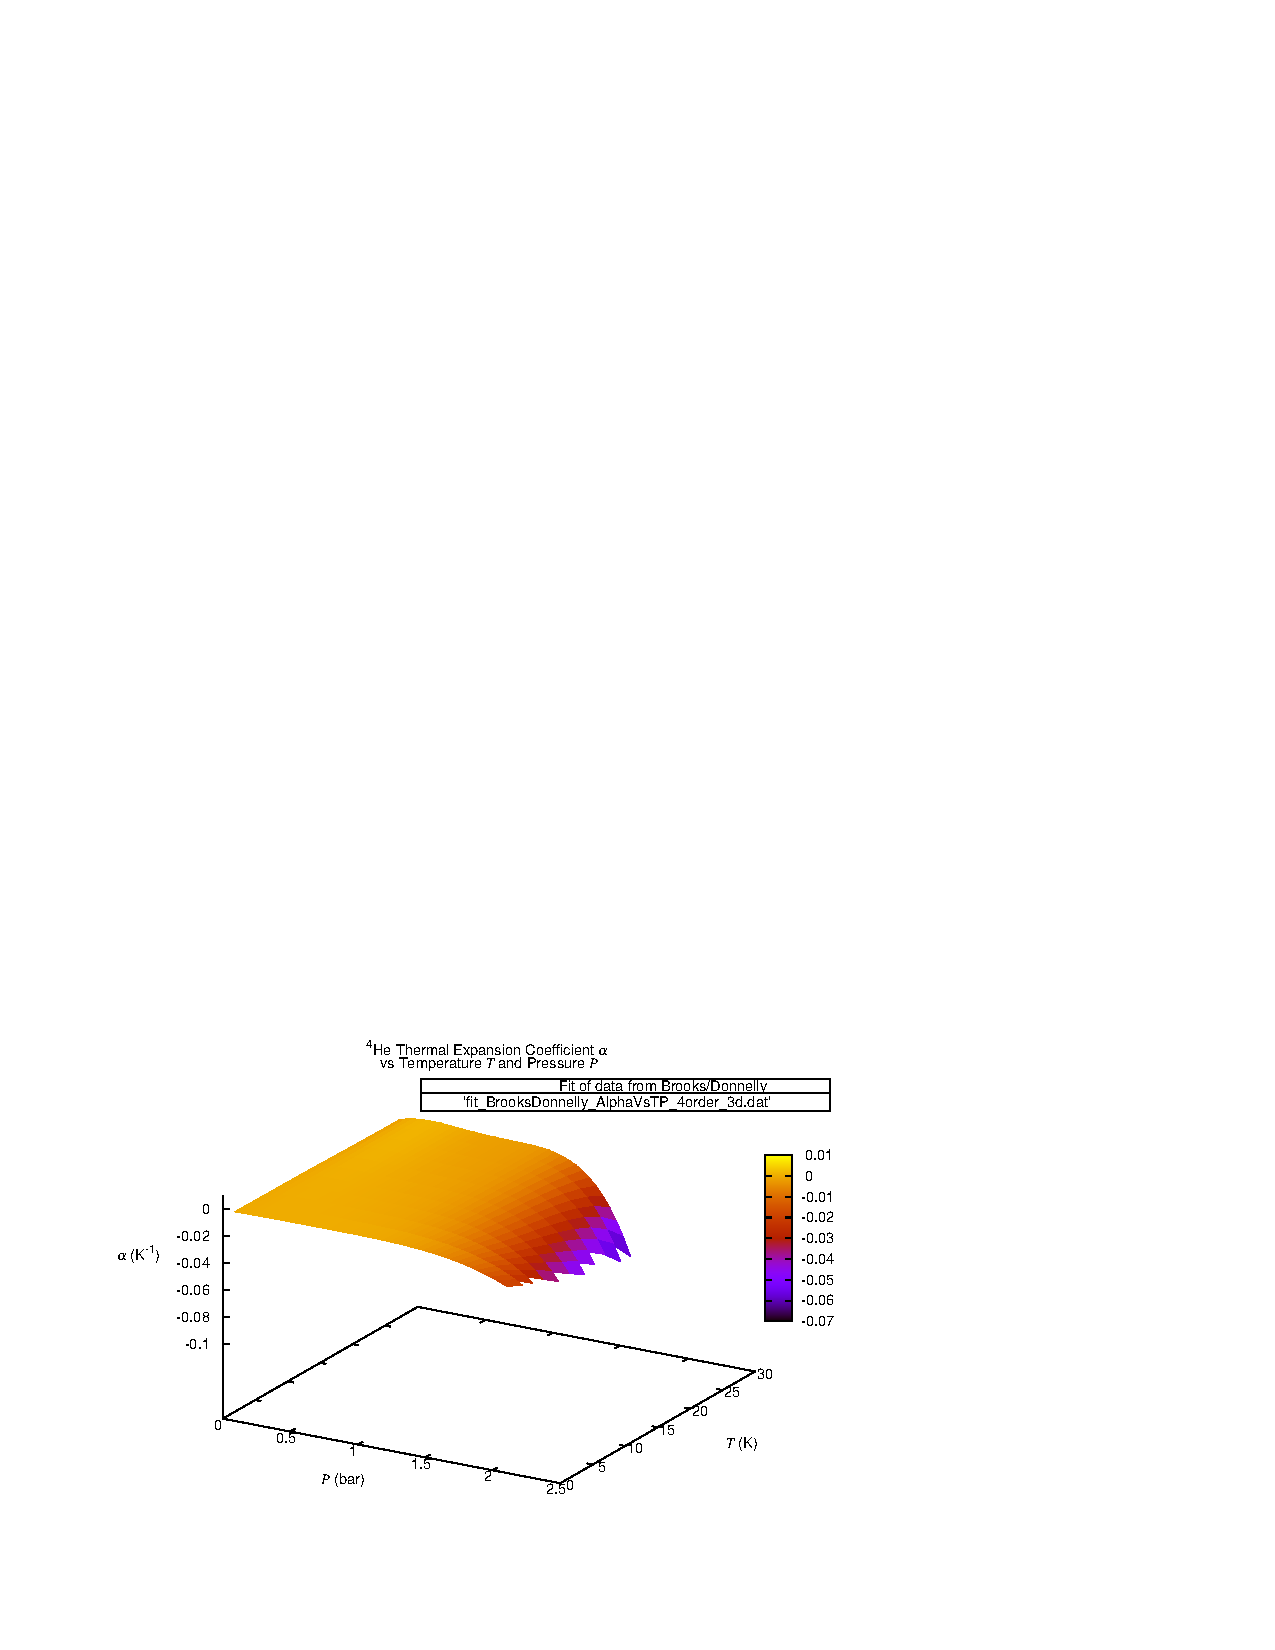
\includegraphics[width=8.5cm,viewport=54 53 410 300]{splot_fit_BrooksDonnelly_AlphaVsTP_4order.pdf}\newline
  \verb|splot_fit_BrooksDonnelly_AlphaVsTP_|\newline
  \verb|4order.pdf|
\else
  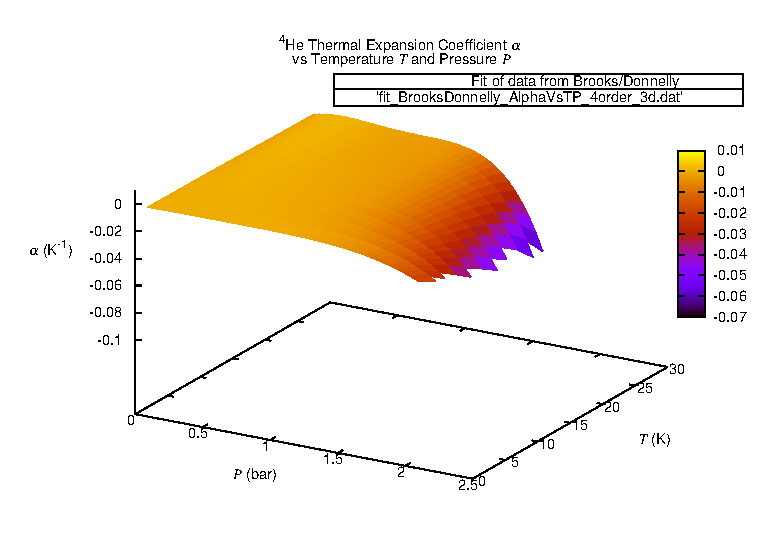
\includegraphics[width=8.5cm]{splot_fit_BrooksDonnelly_AlphaVsTP_4order.ps}\newline
  \verb|splot_fit_BrooksDonnelly_AlphaVsTP_|\newline
  \verb|4order.ps|
\fi
&
\ifpdf
  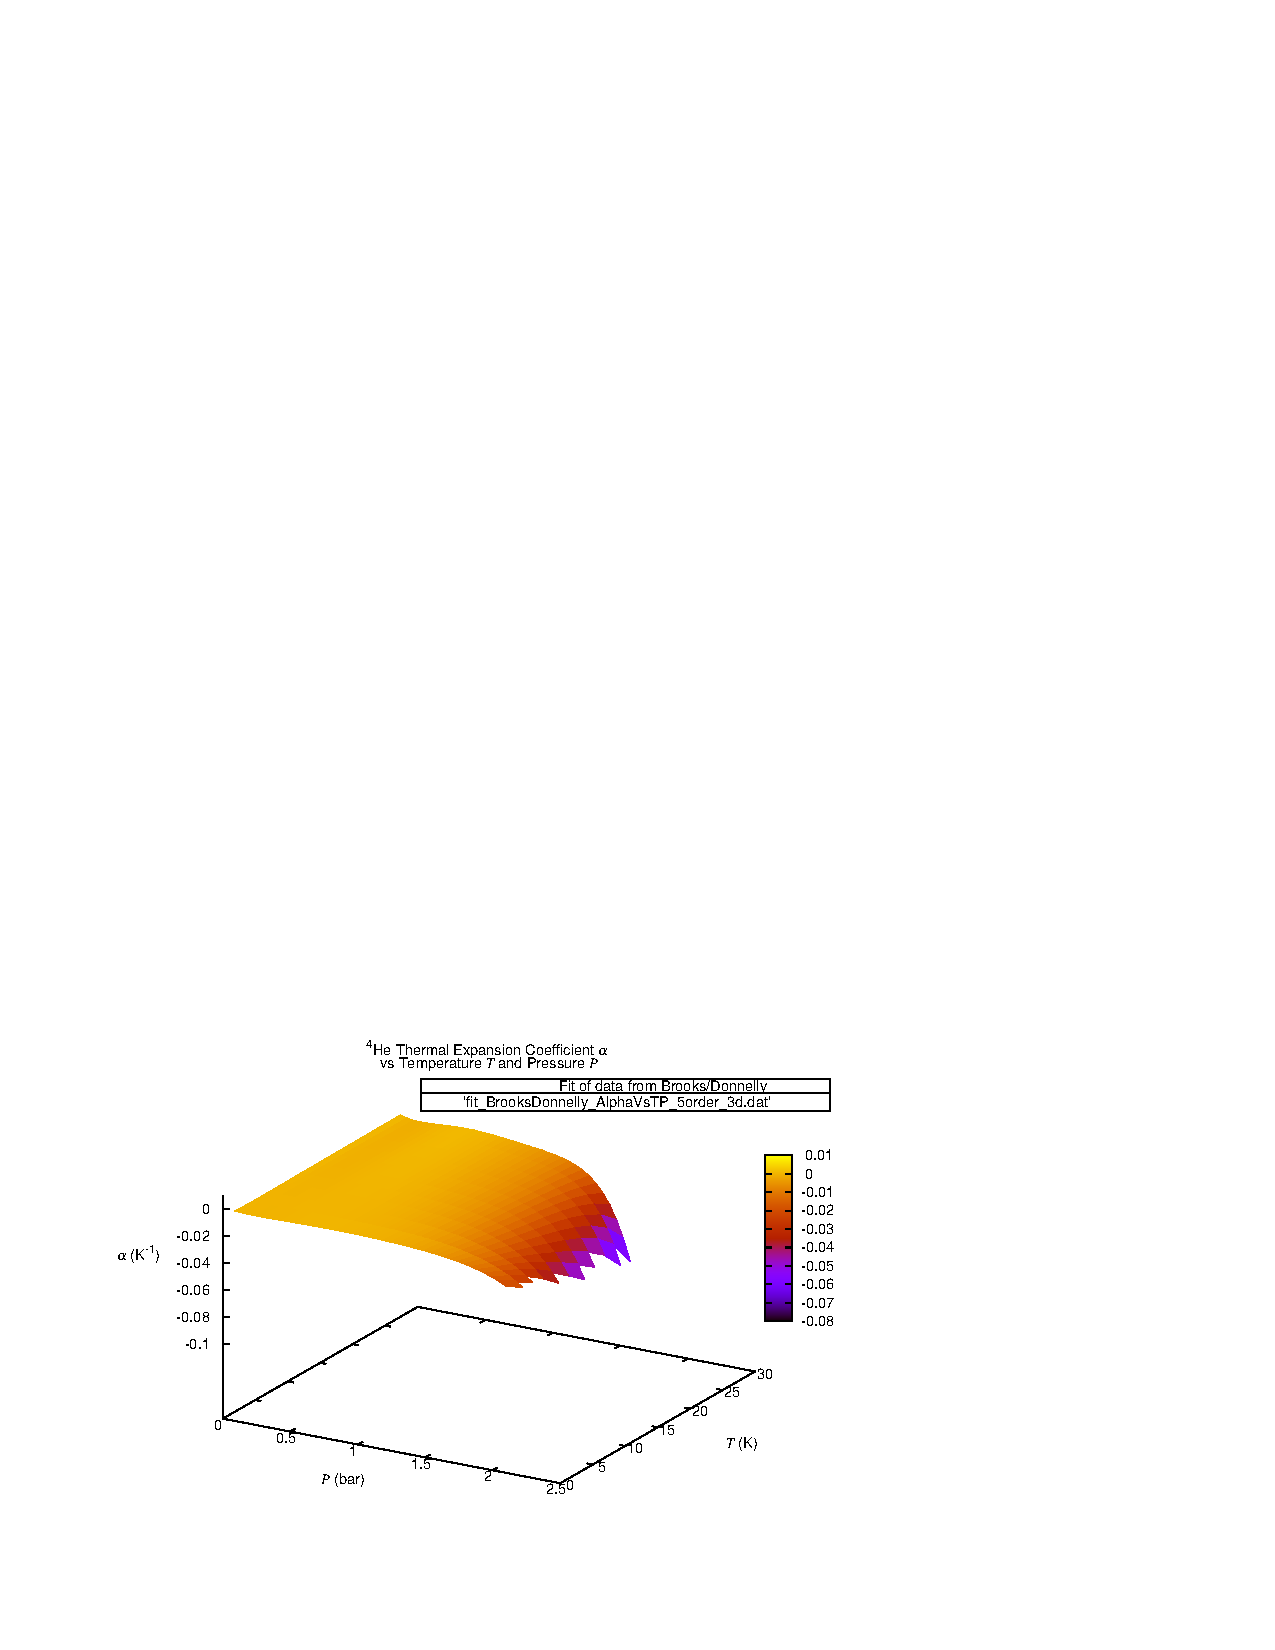
\includegraphics[width=8.5cm,viewport=54 53 410 300]{splot_fit_BrooksDonnelly_AlphaVsTP_5order.pdf}\newline
  \verb|splot_fit_BrooksDonnelly_AlphaVsTP_|\newline
  \verb|5order.pdf|
\else
  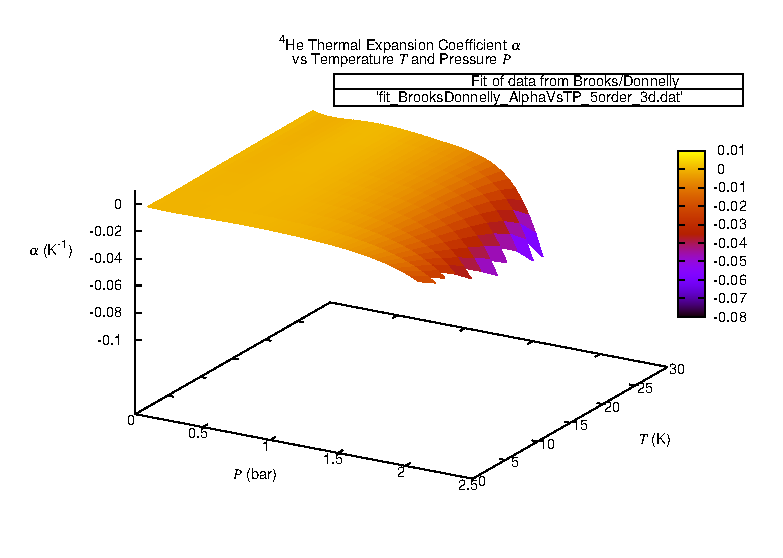
\includegraphics[width=8.5cm]{splot_fit_BrooksDonnelly_AlphaVsTP_5order.ps}\newline
  \verb|splot_fit_BrooksDonnelly_AlphaVsTP_|\newline
  \verb|5order.ps|
\fi
 \\
\ifpdf
  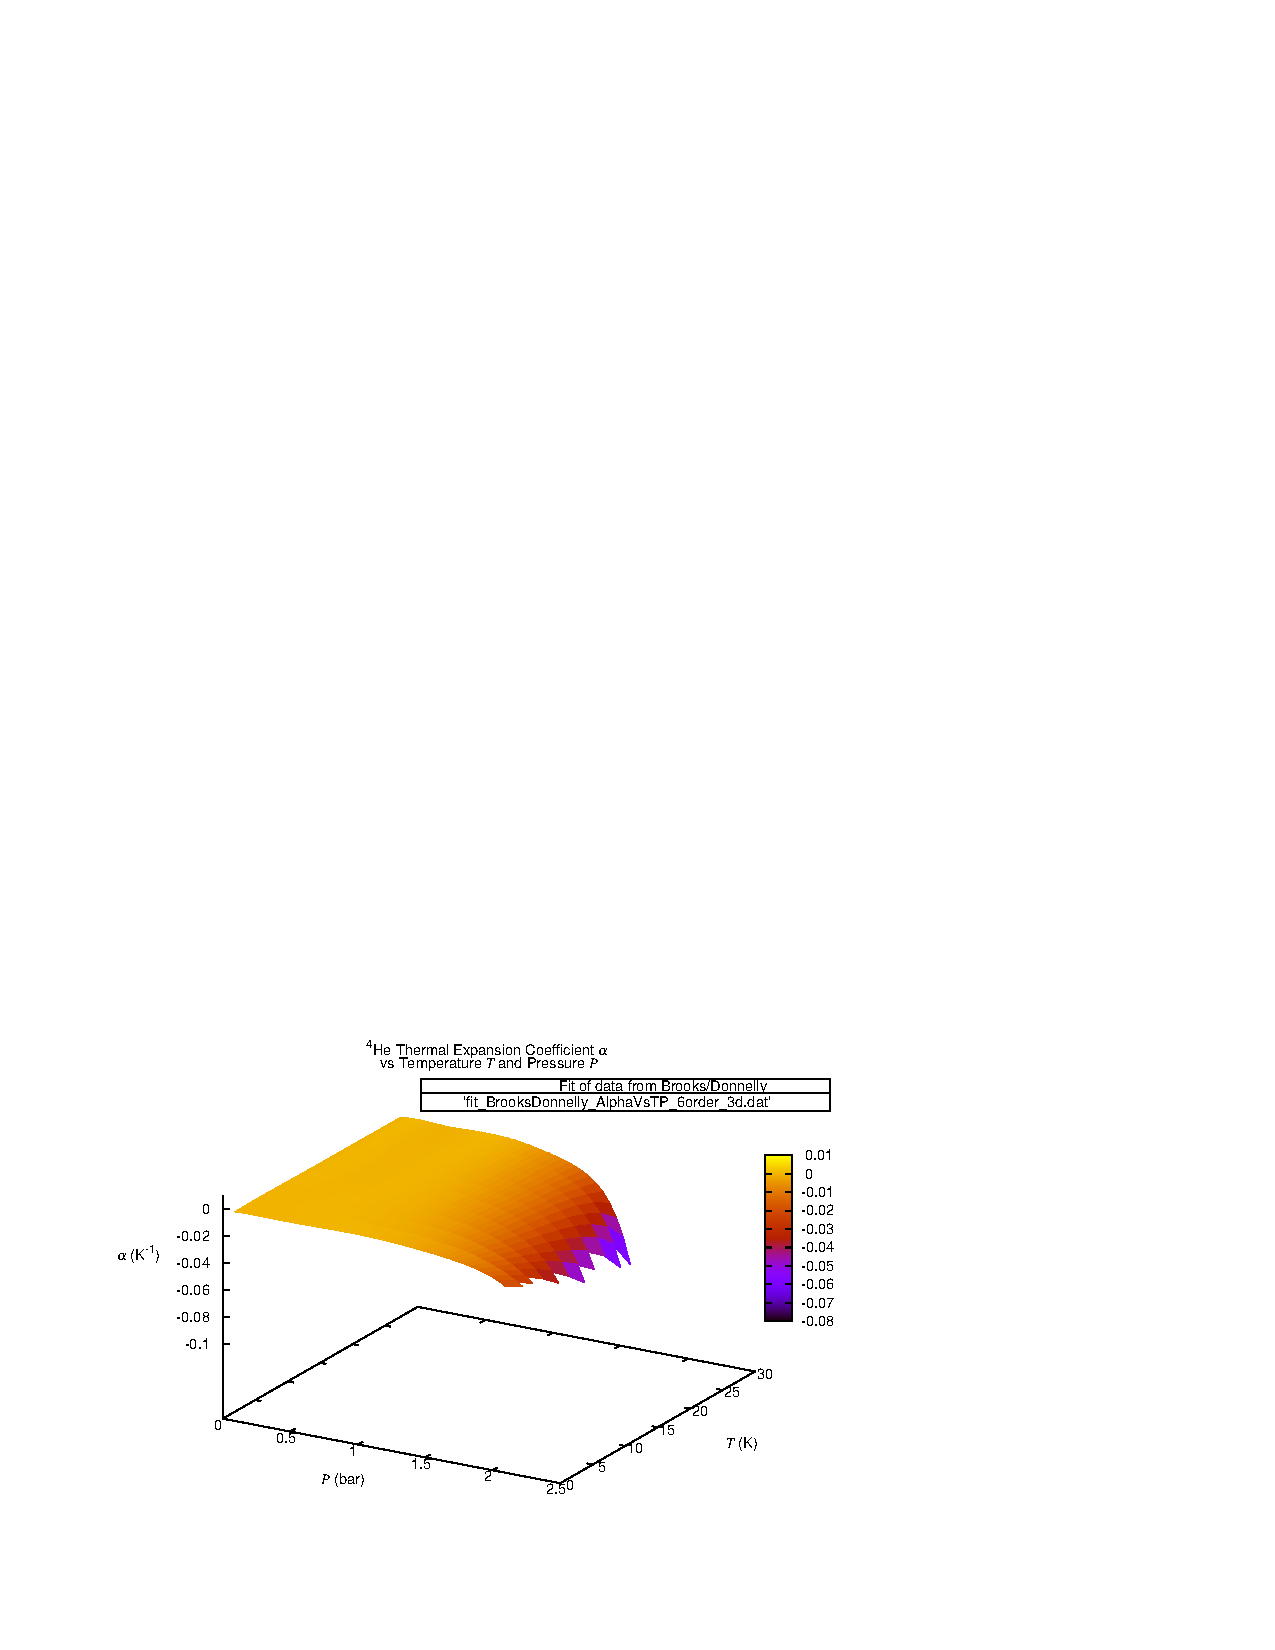
\includegraphics[width=8.5cm,viewport=54 53 410 300]{splot_fit_BrooksDonnelly_AlphaVsTP_6order.pdf}\newline
  \verb|splot_fit_BrooksDonnelly_AlphaVsTP_|\newline
  \verb|6order.pdf|
\else
  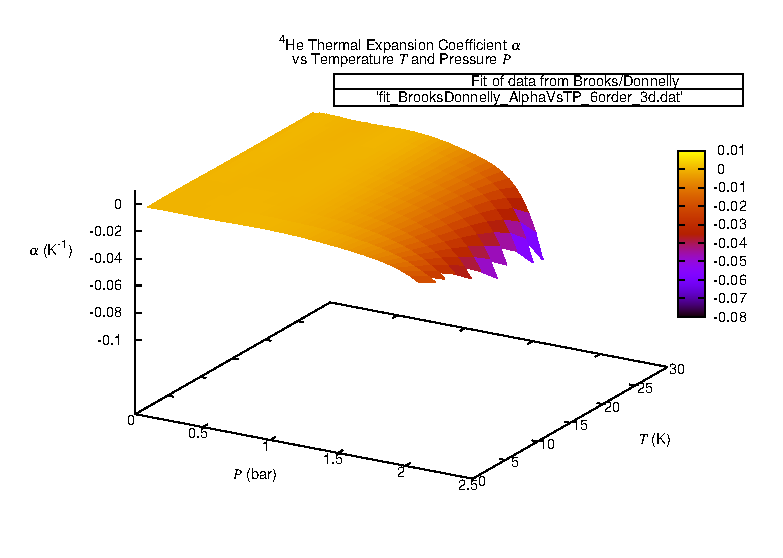
\includegraphics[width=8.5cm]{splot_fit_BrooksDonnelly_AlphaVsTP_6order.ps}\newline
  \verb|splot_fit_BrooksDonnelly_AlphaVsTP_|\newline
  \verb|6order.ps|
\fi
&
 \\
\end{tabular}
\end{center}


\begin{center}
\begin{tabular}[\textwidth]{p{8.5cm}p{8.5cm}}
\ifpdf
  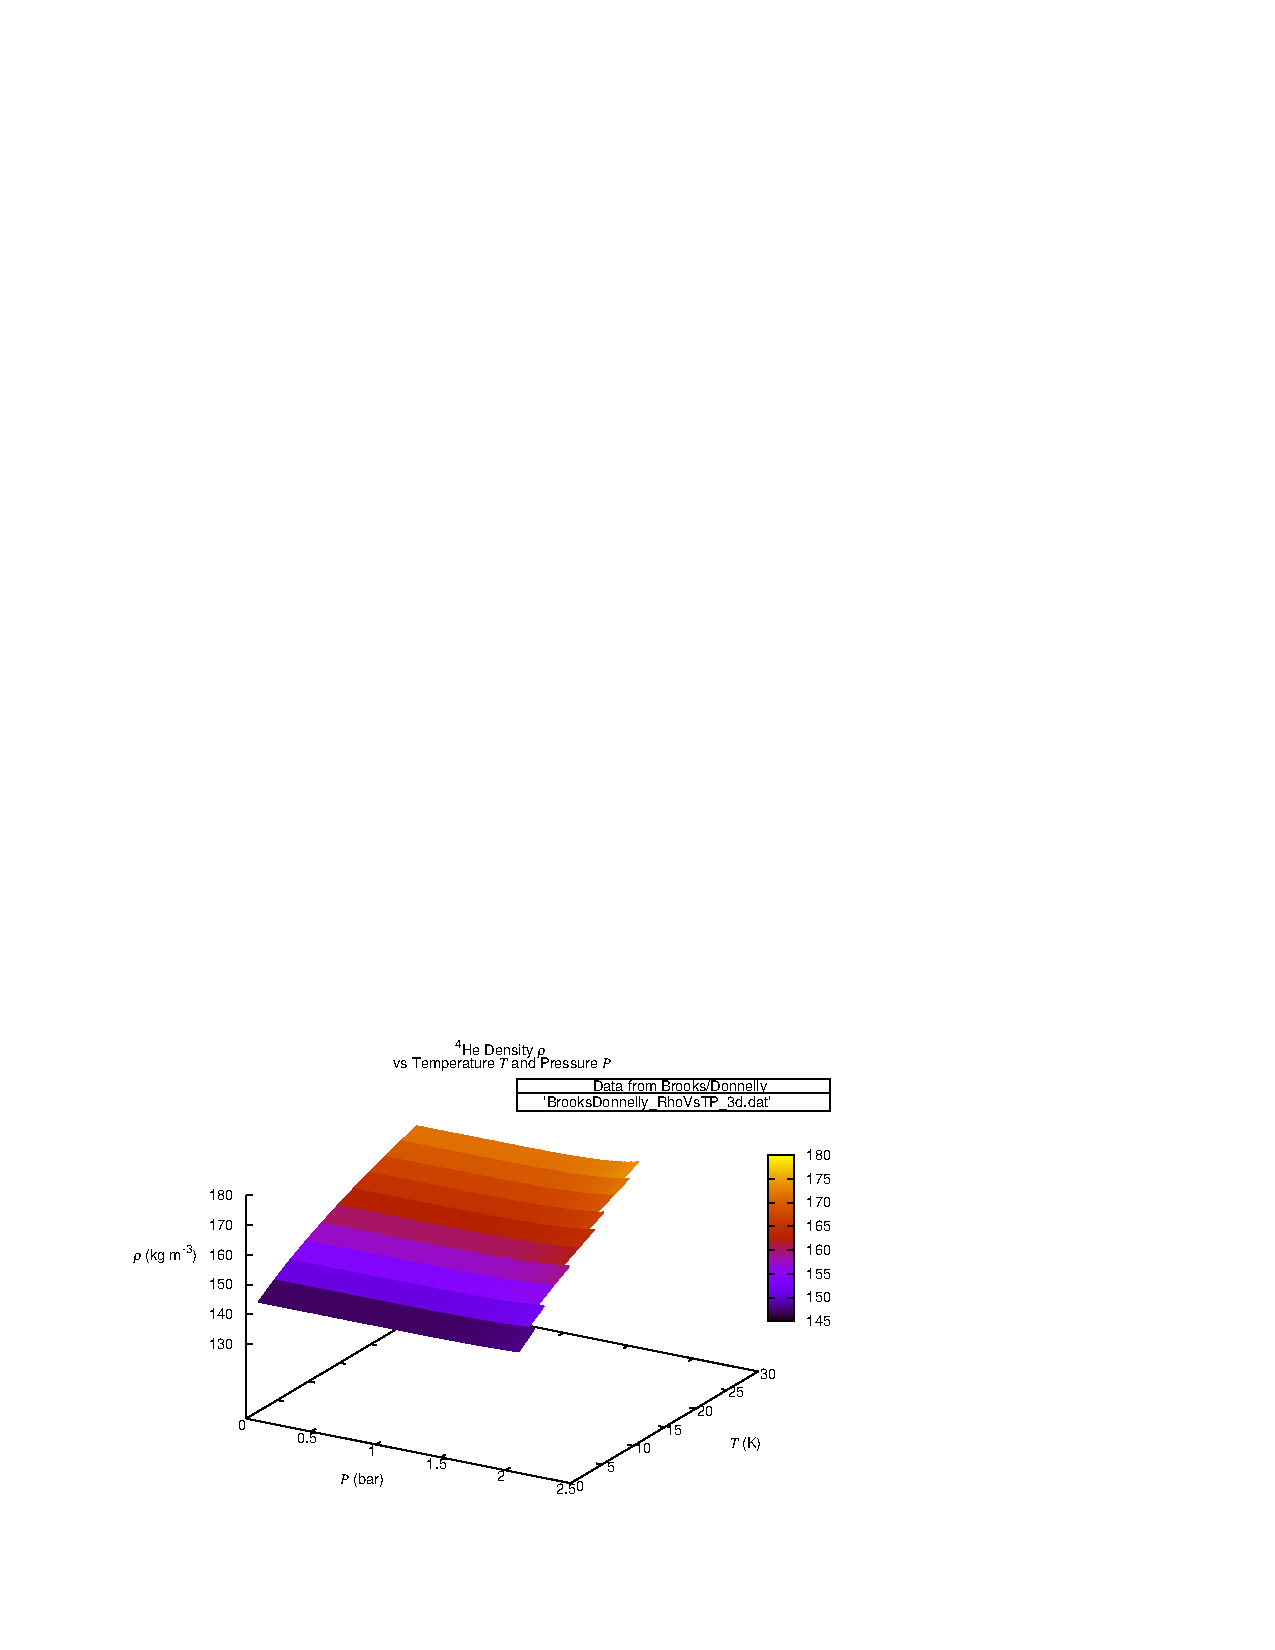
\includegraphics[width=8.5cm,viewport=54 53 410 300]{splot_BrooksDonnelly_RhoVsTP.pdf}\newline
  \verb|splot_BrooksDonnelly_RhoVsTP.pdf|
\else
  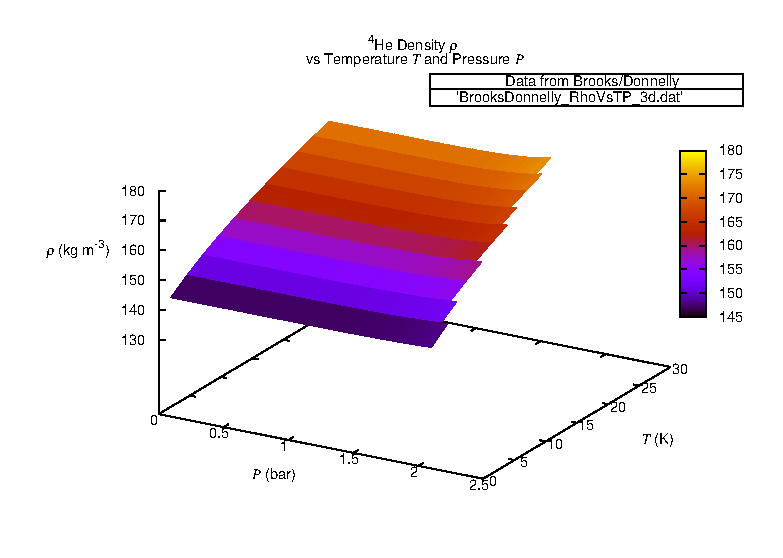
\includegraphics[width=8.5cm]{splot_BrooksDonnelly_RhoVsTP.ps}\newline
  \verb|splot_BrooksDonnelly_RhoVsTP.ps|
\fi
&
\ifpdf
  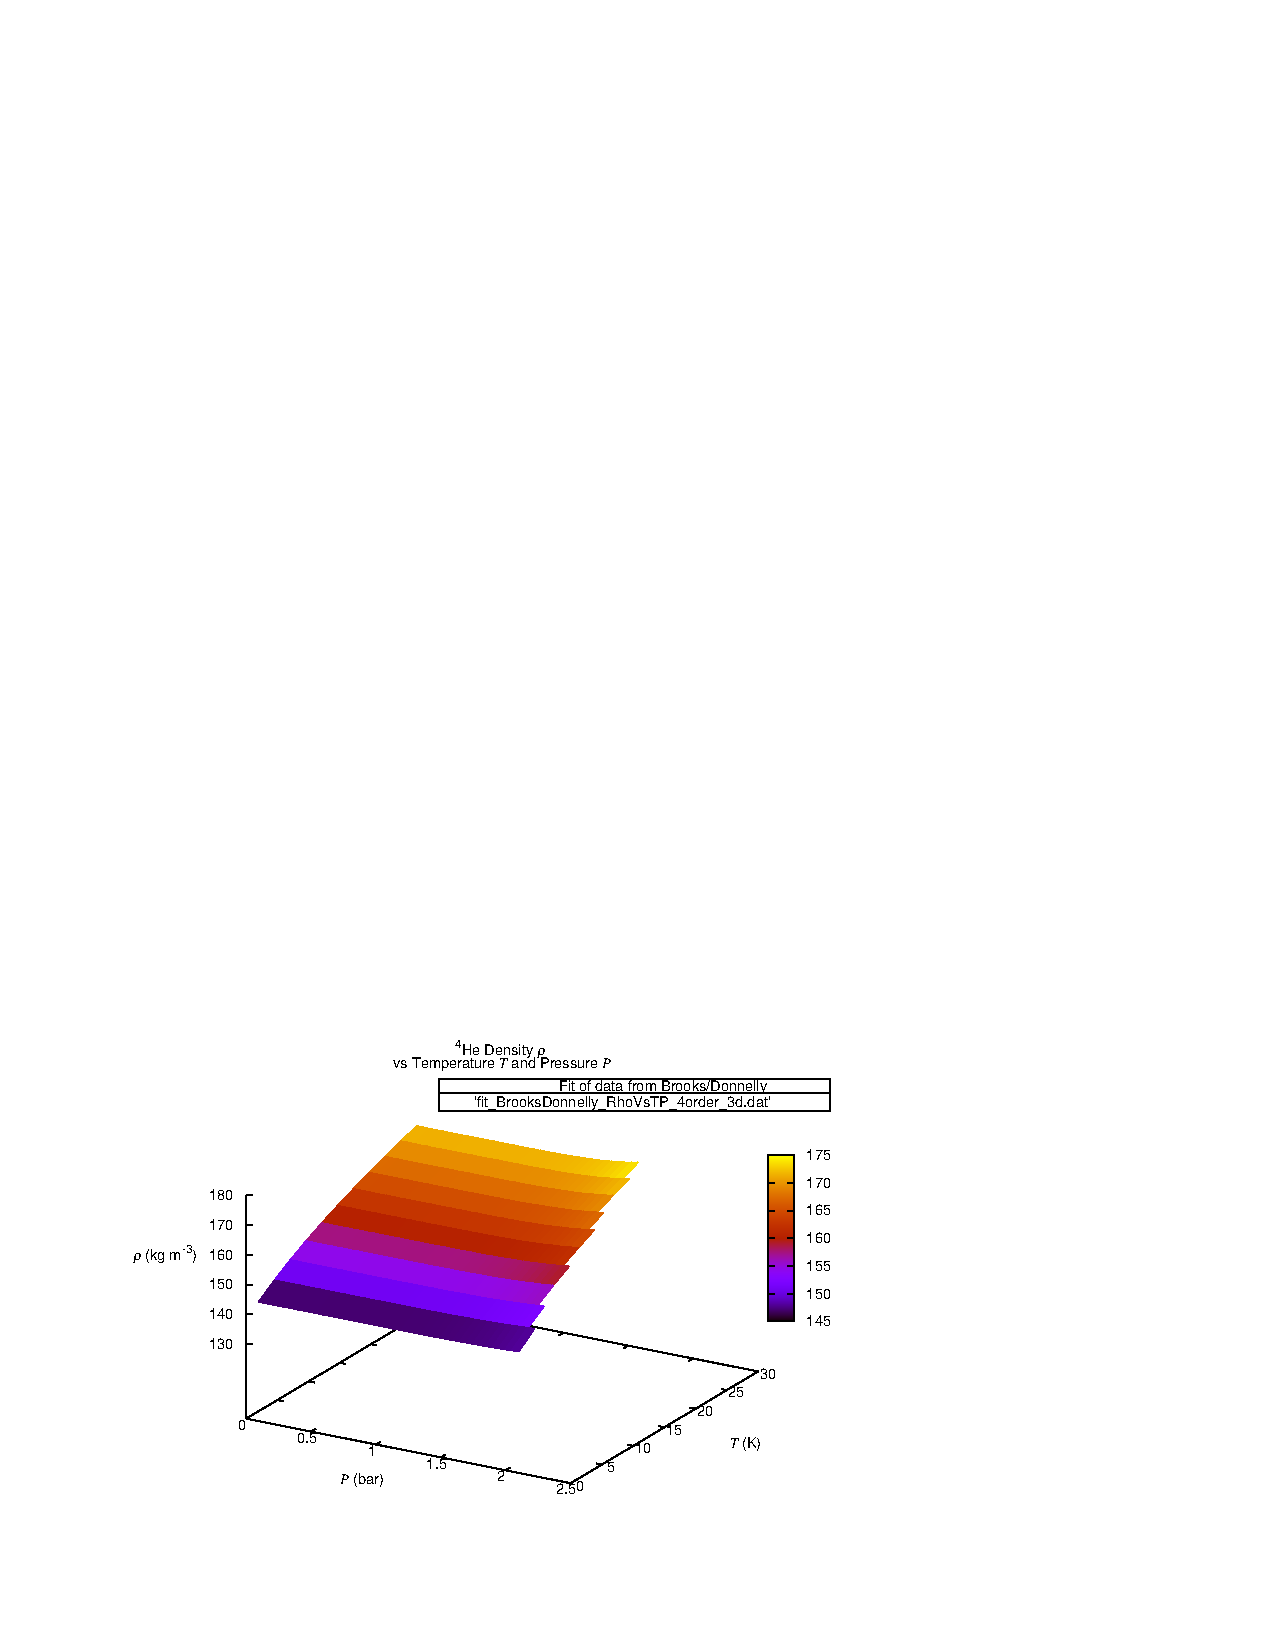
\includegraphics[width=8.5cm,viewport=54 53 410 300]{splot_fit_BrooksDonnelly_RhoVsTP_4order.pdf}\newline
  \verb|splot_fit_BrooksDonnelly_RhoVsTP_|\newline
  \verb|4order.pdf|
\else
  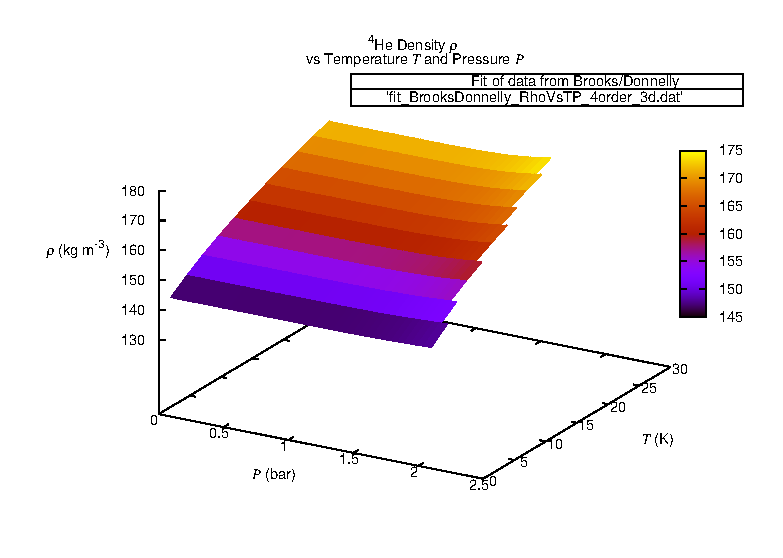
\includegraphics[width=8.5cm]{splot_fit_BrooksDonnelly_RhoVsTP_4order.ps}\newline
  \verb|splot_fit_BrooksDonnelly_RhoVsTP_|\newline
  \verb|4order.ps|
\fi
 \\
\end{tabular}
\end{center}


\newpage
\section{Roton Energy Gap Plots}

In PDF only.

\ifpdf
\begin{center}
\begin{tabular}[\textwidth]{p{8.5cm}p{8.5cm}}
\ifpdf
  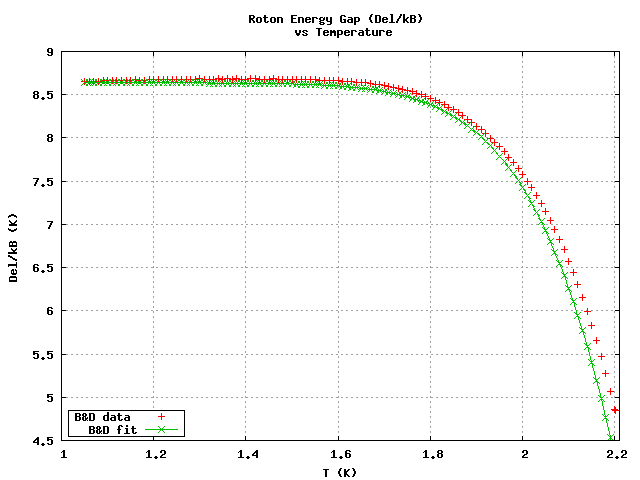
\includegraphics[width=8.5cm]{plot_DelokFit0.png}\newline
  \verb|plot_DelokFit0.png|
\else
  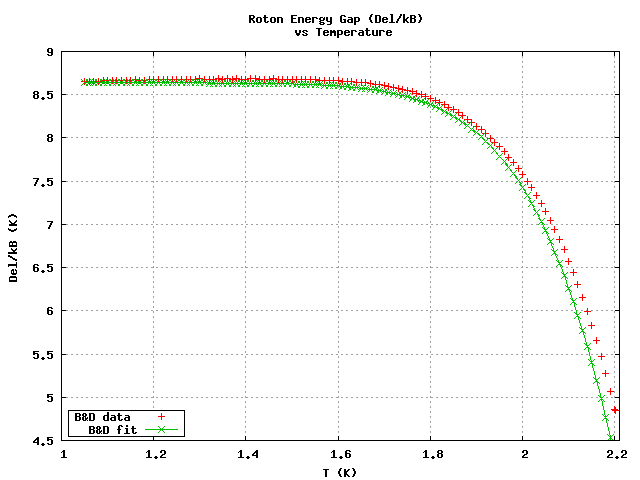
\includegraphics[width=8.5cm]{plot_DelokFit0}\newline % .epsf
  \verb|plot_DelokFit0.epsf|
\fi
&
\ifpdf
  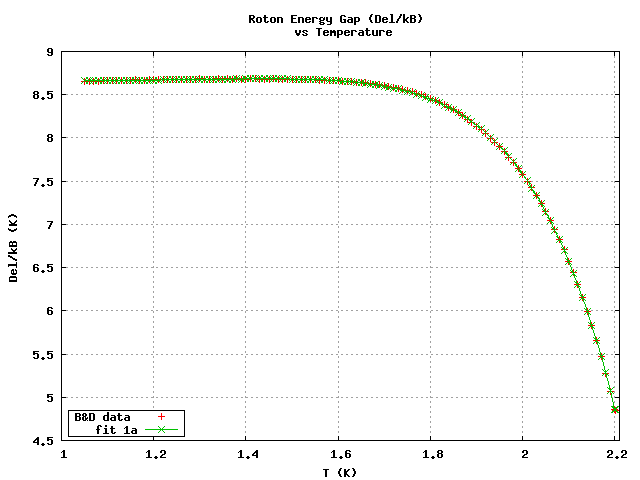
\includegraphics[width=8.5cm]{plot_DelokFit1.png}\newline
  \verb|plot_DelokFit1.png|
\else
  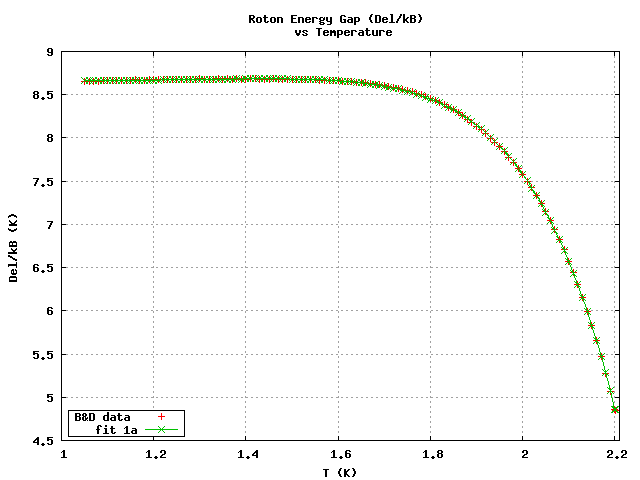
\includegraphics[width=8.5cm]{plot_DelokFit1}\newline % .epsf
  \verb|plot_DelokFit1.epsf|
\fi
 \\
\ifpdf
  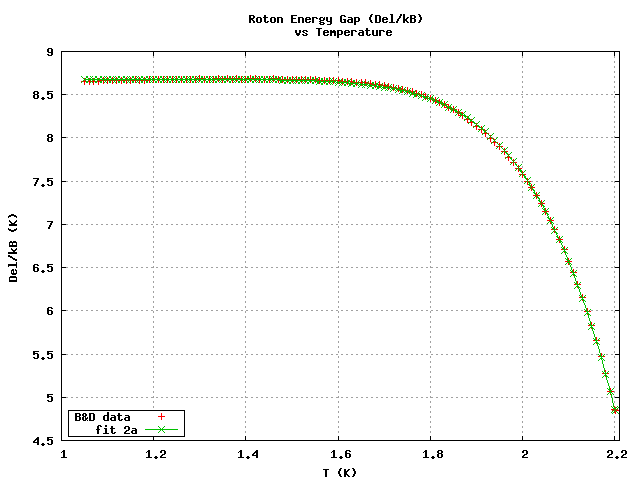
\includegraphics[width=8.5cm]{plot_DelokFit2.png}\newline
  \verb|plot_DelokFit2.png|
\else
  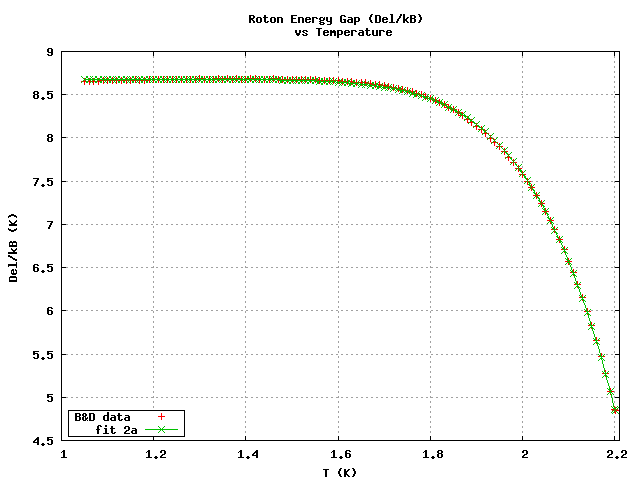
\includegraphics[width=8.5cm]{plot_DelokFit2}\newline % .epsf
  \verb|plot_DelokFit2.epsf|
\fi
&
\ifpdf
  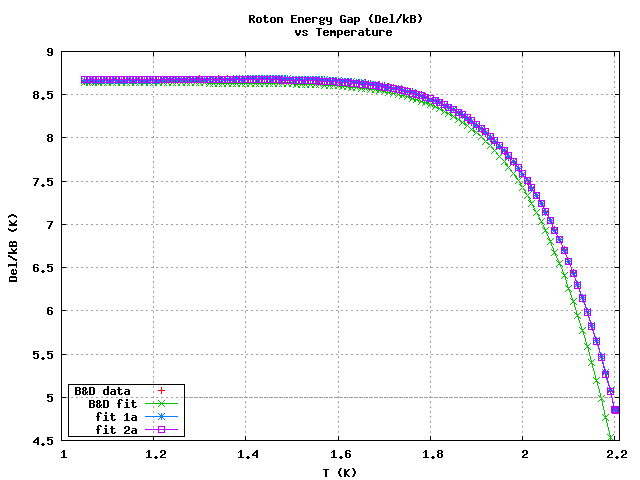
\includegraphics[width=8.5cm]{plot_DelokFits.png}\newline
  \verb|plot_DelokFits.png|
\else
  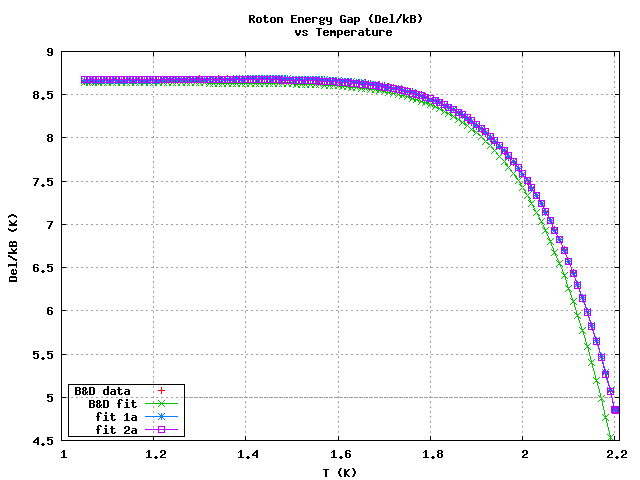
\includegraphics[width=8.5cm]{plot_DelokFits}\newline % .epsf
  \verb|plot_DelokFits.epsf|
\fi
 \\
\end{tabular}
\end{center}
\fi



\end{document}